\documentclass[10pt,twocolumn,oneside]{article}
\setlength{\columnsep}{10pt}                    %兩欄模式的間距
\setlength{\columnseprule}{0pt}                 %兩欄模式間格線粗細

\usepackage{amsthm}								%定義,例題
\usepackage{amssymb}
\usepackage{fontspec}							%設定字體
\usepackage{color}
\usepackage[x11names]{xcolor}
\usepackage{listings}							%顯示code用的
\usepackage{fancyhdr}							%設定頁首頁尾
\usepackage{graphicx}							%Graphic
\usepackage{enumerate}
\usepackage{titlesec}
\usepackage{amsmath}
\usepackage[CheckSingle, CJKmath]{xeCJK}
 \usepackage{CJKulem}
\usepackage{tikz}

\usepackage{multicol}
\usepackage{graphicx}

\usepackage{amsmath, courier, listings, fancyhdr, graphicx}
\topmargin=0pt
\headsep=5pt
\textheight=740pt
\footskip=0pt
\voffset=-50pt
\textwidth=545pt
\marginparsep=0pt
\marginparwidth=0pt
\marginparpush=0pt
\oddsidemargin=0pt
\evensidemargin=0pt
\hoffset=-42pt

%\renewcommand\listfigurename{圖目錄}
%\renewcommand\listtablename{表目錄}

%%%%%%%%%%%%%%%%%%%%%%%%%%%%%

\setmainfont{Consolas}
\setmonofont{Consolas}
\setCJKmainfont{Noto Sans CJK TC}
\XeTeXlinebreaklocale "zh"						%中文自動換行
\XeTeXlinebreakskip = 0pt plus 1pt				%設定段落之間的距離
\setcounter{secnumdepth}{3}						%目錄顯示第三層

%%%%%%%%%%%%%%%%%%%%%%%%%%%%%
\makeatletter
\lst@CCPutMacro\lst@ProcessOther {"2D}{\lst@ttfamily{-{}}{-{}}}
\@empty\z@\@empty
\makeatother
\lstset{										% Code顯示
    language=C++,									% the language of the code
    basicstyle=\footnotesize\ttfamily, 					% the size of the fonts that are used for the code
    %numbers=left,									% where to put the line-numbers
    numberstyle=\footnotesize,					% the size of the fonts that are used for the line-numbers
    stepnumber=1,									% the step between two line-numbers. If it's 1, each line  will be numbered
    numbersep=5pt,									% how far the line-numbers are from the code
    backgroundcolor=\color{white},				% choose the background color. You must add \usepackage{color}
    showspaces=false,								% show spaces adding particular underscores
    showstringspaces=false,						% underline spaces within strings
    showtabs=false,								% show tabs within strings adding particular underscores
    frame=false,										% adds a frame around the code
    tabsize=2,										% sets default tabsize to 2 spaces
    captionpos=b,									% sets the caption-position to bottom
    breaklines=true,								% sets automatic line breaking
    breakatwhitespace=false,						% sets if automatic breaks should only happen at whitespace
    escapeinside={\%*}{*)},						% if you want to add a comment within your code
    morekeywords={*},								% if you want to add more keywords to the set
    keywordstyle=\bfseries\color{Blue1},
    commentstyle=\itshape\color{Red4},
    stringstyle=\itshape\color{Green4},
}

\graphicspath{ {./img/} }

\titlespacing{\section}{0pt}{0pt}{0pt}
\titlespacing{\subsection}{0pt}{0pt}{0pt}
\titlespacing{\subsubsection}{0pt}{0pt}{0pt}

\begin{document}
\pagestyle{fancy}
\fancyfoot{}
\fancyhead[C]{National Chiao Tung University}
\fancyhead[L]{NCTU\_Revue}
\fancyhead[R]{(\today) Page \thepage}
\renewcommand{\headrulewidth}{0.4pt}
\renewcommand{\contentsname}{Contents}

\scriptsize
\begin{multicols}{2}
\tableofcontents
\end{multicols}

\section{vimrc}
	\lstinputlisting [language=c++] { Basic/vimrc }
\begin{center}
    
\includegraphics[width=70mm]{capoo.png}
\end{center}

\newpage
\input{content.tex}
\section{Notes}
    \subsection{Burnside's Lemma}
        \large $\left | X / G \right | = \frac{1}{\left | G \right |}\sum_{g \in G}\left | X^g \right |$
    \subsection{Pick's Theorem}
        \large $A = i + \frac{b}{2} - 1$
        \small
        \begin{itemize}
            \item $A$: Area
            \item $i$: \# of interior points
            \item $b$: \# of boundary points
        \end{itemize}
    \subsection{Lucas's Theorem}
        \large $\binom{m}{n}\equiv \prod_{i=0}^k \binom{m_i}{n_i} (mod p)$
        \small
        \begin{itemize}
            \item $m = m_kp^k + m_{k-1}p^{k-1} + \cdots + m_1p + m_0$
            \item $n = n_kp^k + n_{k-1}p^{k-1} + \cdots + n_1p + n_0$
        \end{itemize}

        


\onecolumn
\centering
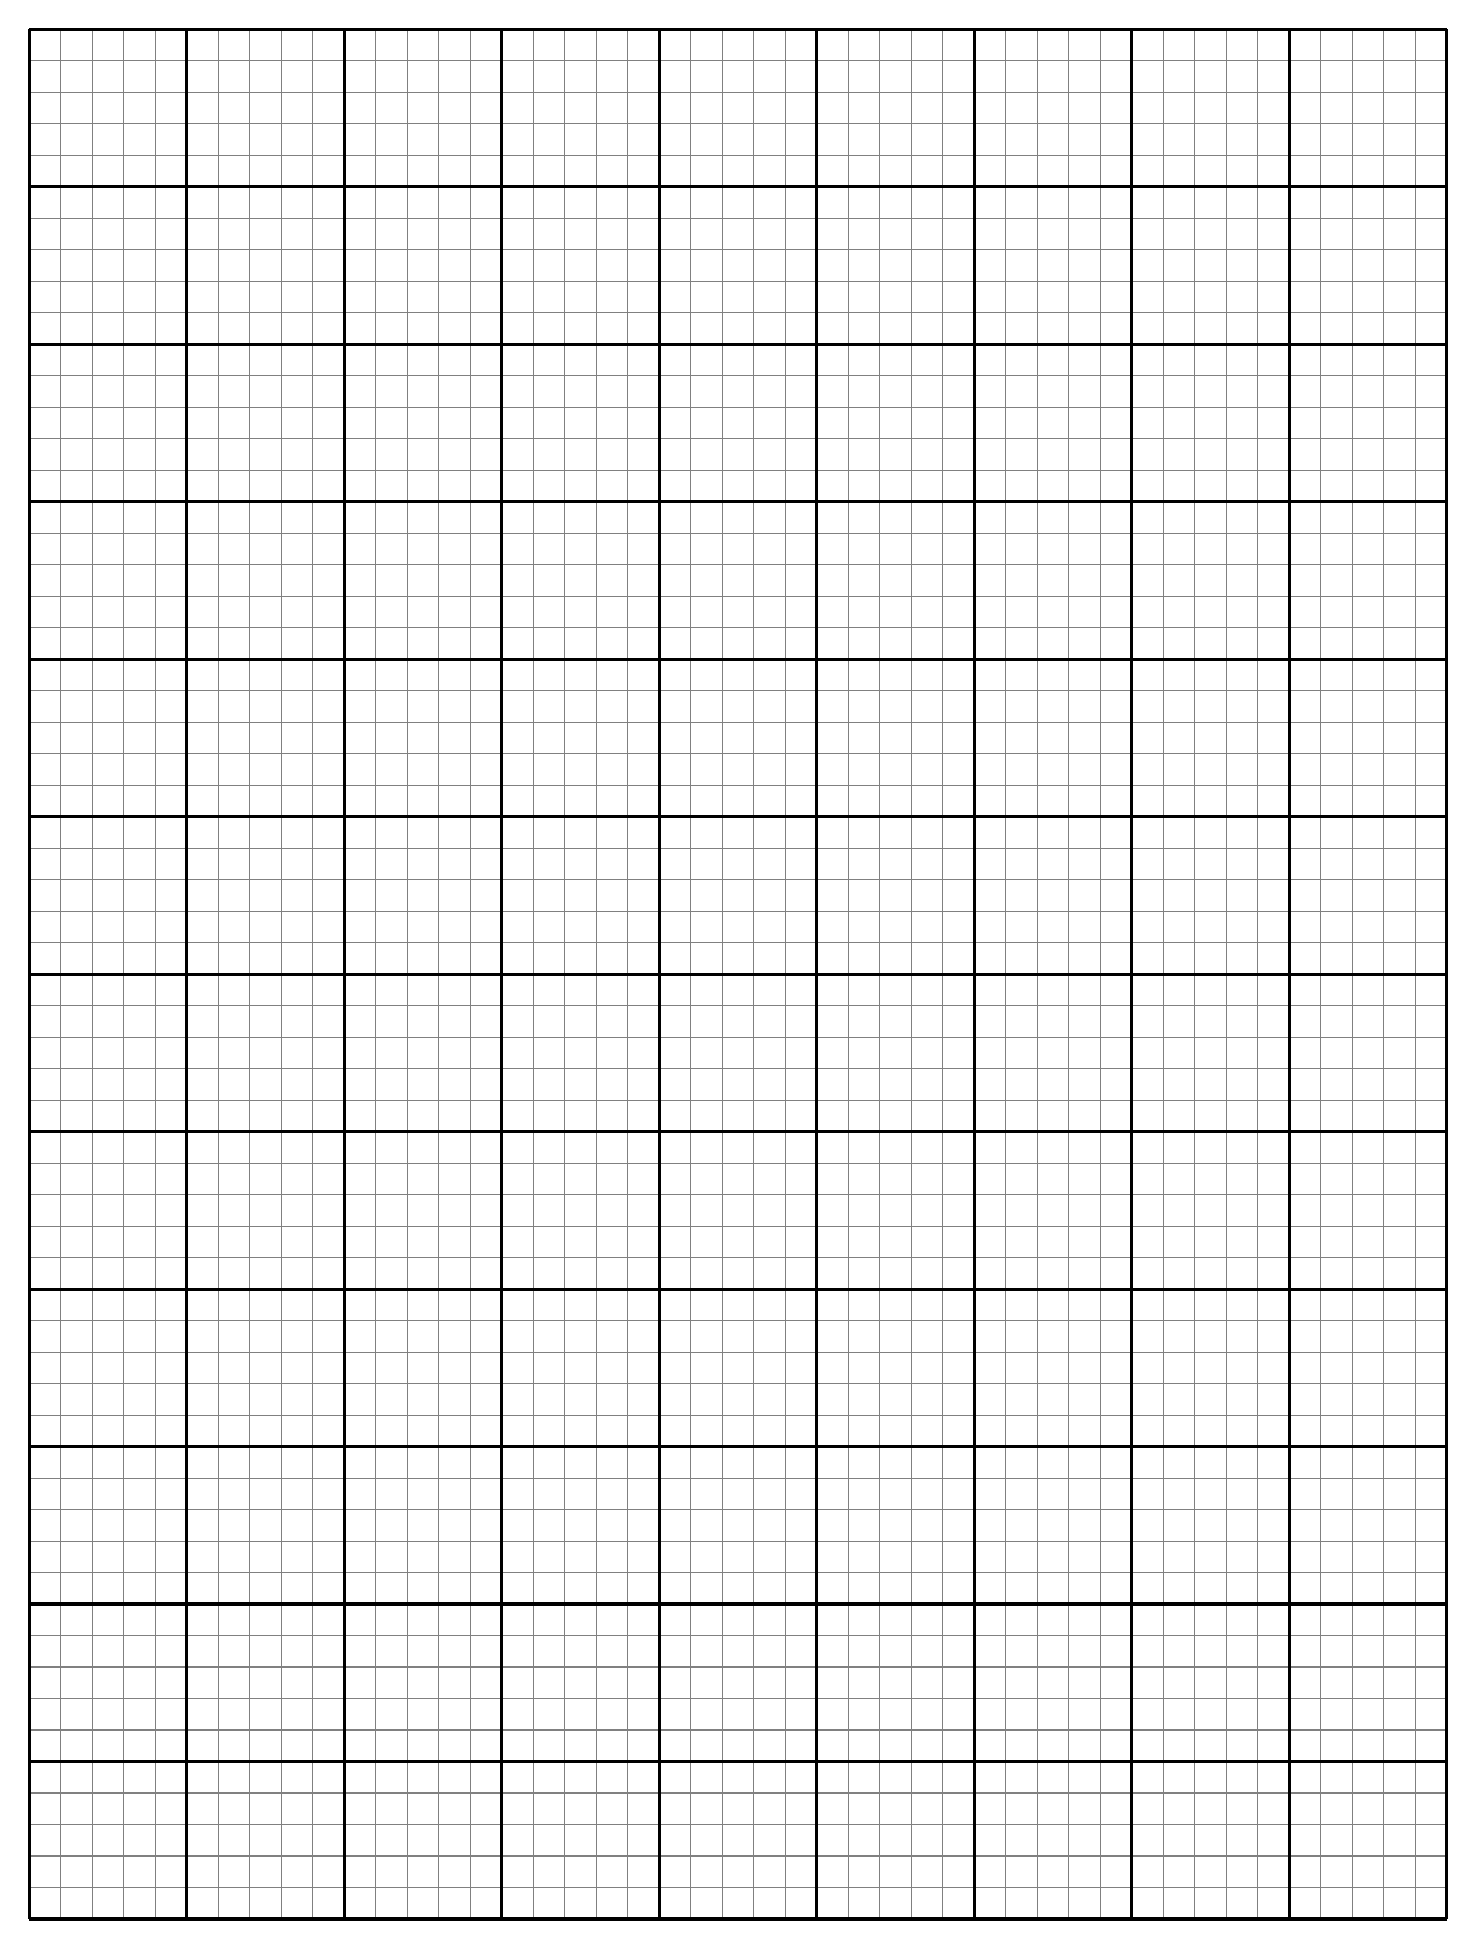
\begin{tikzpicture}[every node/.style={minimum size=1cm-\pgflinewidth, outer sep=10pt}, scale=2]
    \draw[step=0.2cm,color=gray] (0,0) grid (9,12);
    \draw[step=1cm,color=black,line width=0.4mm] (0,0) grid (9,12);

\end{tikzpicture}
\end{document}
